\chapter{PACORA Implementation in a Manycore Operating System}\label{tess_design_ch}
\section{Response Time Model Creation}\label{rtf_creation}
To create RTF models either at install time or online we use a convex
least-squares approach described below.  At install time, we use a
genetic algorithm, Audze-Eglasis Design of
Experiments\cite{bates-aes03}, to select the resource vectors to use
for training.  These vectors and their response times are fed into the
convex least-squares algorithm. Online model building uses data
from the application's response time history.

\subsection*{Data Collection and Model Creation Time}
There are many ways to collect the response time data for
applications. The user-level runtime scheduler is one possible source,
or the operating system could measure progress using performance
counters.  In our implementation, applications report their own
measured values; however, this solution was chosen simply as a way to
test the validity of the concept.  In a production operating system it
may not be a good idea because applications could lie about their
performance.  In a single-operator datacenter environment this might be less of a concern.

There are also many different possible moments to create response time functions.  RTFs could be created in advance and distributed with the application. This approach could make lots of sense for app stores since most of them cater to just a few platforms. RTFs could also be crowd-sourced and built in the cloud, which has the advantage making it easy to collect a diverse set of training points.  However, all of these approaches lack adaptability.  As a result, we have chosen to implement two solutions that collect data directly from the user's machine.  The first approach is to adapt to the system by collecting all of the training points at application install time and building the model then.  The most highly adaptive approach collects data continuously as the application runs, uses the data to modify the model training set, and rebuilds the model.  A hybrid approach may be the most effective: applications can begin with a generic model and improve it over time. The remainder of this Section describes our model creation process in detail.

In a client operating system, management of penalty function modifications
should be highly automated by the system to avoid unduly burdening the user.
As an application grows or diminishes in importance, its penalty function can be modified accordingly.
Adjustment is also likely to occur in transitions between operating scenarios.
For example, when unplugging a device all of the background activities could have their slopes significantly reduced to save battery life.

\subsection*{Least-Squares Minimization}
After enough measurements, discovery of the model parameters $w$ that define the function $\tau$
can be based on a solution to the over-determined linear system $t=Dw$,
where $t$ is a column vector of actual response times measured for the application
and $D$ is a matrix whose $i$th row $D_{i,*}$ contains the corresponding resource vector.
Estimating $w$ is relatively straightforward: a least-squares solution accomplished via
\emph{QR factorization}\cite{GoVL} of $D$ will determine the $w$ that minimizes the \emph residual error of
$\|Dw - t\|^2_2 =  \|Rw - Q^Tt\|^2_2$.
%The solution proceeds as follows:
%\begin{eqnarray*}
%t     &=& Dw  - \varepsilon    \\
%      &=& QRw - \varepsilon    \\
%Q^Tt  &=& Rw  - Q^T\varepsilon
%\end{eqnarray*}
%
The individual elementary orthogonal transformations, \emph{e.g.,} Givens rotations,
that triangularize $R$ by progressively zeroing out $D$'s sub-diagonal elements are simultaneously applied to $t$.
%The elements of the resulting vector $Q^Tt$ that correspond to zero rows in $R$ comprise $-Q^T\varepsilon$.
%Since $Rw$ exactly equals the upper part of $Q^Tt$, the upper part of $Q^T\varepsilon$ is zero. The residual error for the %$t_i$
%can be found by premultiplying $Q^T\varepsilon$ by $Q$.

%This formulation assumes a model norm $p = 1$. If a different model norm $p$ is desired, such as $p = 2$, we could first square %each measurement in $t$
%and each reciprocal bandwidth term in $D$ and then follow the foregoing procedure.
%The elements of the result $w$ will be squares as well, and the 2-norm of the difference in the squared quantities will be %minimized.  This is not the same as minimizing the 4-norm; what is being minimized is $1/2\|\mbox{diag}(Dww^TD^T - tt^T)\|^2_2$.

\subsection{On-line Response Time Modeling}
As resource allocation continues, more measurements will become available to augment $t$ and $D$.
Moreover, older data may poorly represent the current behavior of the application.
\pacora uses an incremental approach described below to replace old data and efficiently update RTFs.

\subsubsection*{Incremental Least-Squares}
What is needed is a factorization $\tilde{Q}\tilde{R}$ of a new matrix $\tilde{D}$
derived from $D$ by dropping a row, perhaps from the bottom,
and adding a row, perhaps at the top.
Corresponding elements of $t$ are dropped and added to form $\tilde{t}$.

The matrices $\tilde{Q}$ and $\tilde{R}$ can be generated by applying Givens rotations
as described in Section 12 of \cite{GoVL} to \emph{downdate} or \emph{update} the factorization
much more cheaply than recomputing it \emph{ab initio}.
The method requires retention and maintenance of $Q^T$ but not of $D$.
Every update in \pacora is preceded by a downdate that makes room for it.
Downdated rows are \emph{not} always the oldest (bottom) ones, but
an update always adds a new top row.
For several reasons, the number of rows $m$ in $R$
will be at least twice the number of columns $n$.
Rows selected for downdating will always be in the lower $m - n$ rows of $R$,
guaranteeing that the most recent $n$ updates are always part of the model.

%\subsubsection*{Non-Negativity}
%\begin{figure*}[!t]
%	\begin{center}	
%%		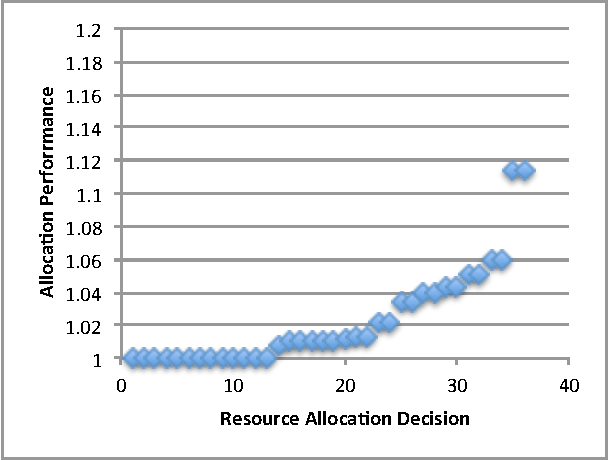
\includegraphics[width=.45\textwidth]{cluster_decision_points.pdf}
%		\caption{Performance of \pacora's NNLS algorithm}
%		\label{model_build_perf}
%	\end{center}
%\end{figure*}

To guarantee convexity of the RTF, the solution $w$ to $t \approx QRw$ must have no negative components.
Intuitively, when a resource is associated with more than a single $w_j$
or when the measured response time increases with allocation then negative $w_j$ may occur. \emph{Non-negative Least-Squares} problems (NNLS) are common linear algebra, and there are several well-known techniques\cite{ChPl}.
However since \pacora's online model maintenance calls for
incremental downdates and updates to rows of $Q^T$, $Q^Tt$ and $R$,
the NNLS problem is handled with a scheme
based on the \emph{active-set} method\cite{LaHa} that
also downdates and updates the \emph{columns} of $R$ incrementally,
roughly in the spirit of Algorithm~3 in~\cite{LuDu}.
However, \pacora's algorithm cannot ignore downdated columns of $R$
because subsequent \emph{row} updates and downdates must have due effect
on these columns to allow their later reintroduction via column updates as necessary.
This problem is solved by leaving the downdated columns in place,
skipping over them in maintaining and using the QR factorization.

The memory used in maintaining a model with $n$ weights is modest, $24n^2 + 21n + \textrm{O}(1)$ bytes.
For $n = 8$ this is under 2 KB, fitting nicely in L1 cache.
Our NNLS implementation takes \SI{4}{\micro\second} per update-downdate pair in \tess.
%Figure~\ref{model_build_perf} shows the performance of \pacora's NNLS algorithm.

\subsubsection*{Model Rank Preservation}
If care is not taken in downdating $R$, its rows may become so linearly dependent,
perhaps from repetitive resource allocations,
that determining a unique $w$ is impossible.
The rank of $R$ depends on both the resource optimization trajectory and the
choices made in the row downdate-update algorithm.
\pacora exploits the latter idea and simply avoids downdating any row that will make $R$ rank-deficient.

\subsubsection*{Outliers and Phase Changes}

%\begin{figure*}[!t]
%	\begin{center}	
%%		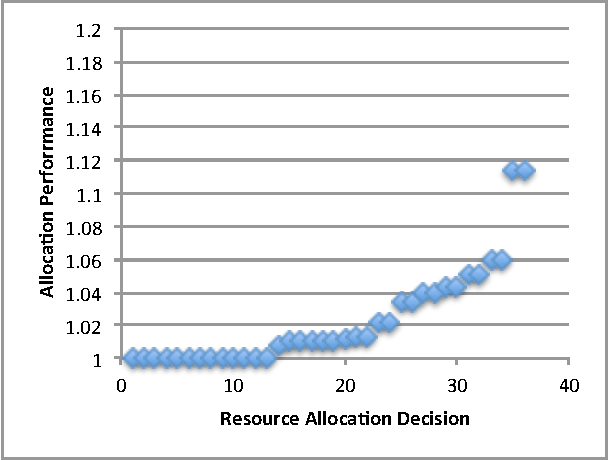
\includegraphics[width=.45\textwidth]{cluster_decision_points.pdf}
%		\caption{\pacora's online model creation algorithm adapting to a video application changing phases}
%		\label{phase_change}
%	\end{center}
%\end{figure*}

Some response time measurements may be ``noisy'' or even erroneous.
A weakness of least-squares modeling is the high importance it gives to outlying values.
On the other hand, when an application changes phase it is important to adapt quickly,
and what looks like an outlier when it first appears may be a harbinger of change.
What is needed is a way to discard either old or outlying data
with a judicious balance between age and anomaly.

The downdating algorithm accomplishes this by weighting the errors in $\varepsilon = Q(Q^Tt - Rw)$
between the predicted response times $\tau$ and the measured ones $t$ by a factor
that increases exponentially with the age $g(i)$ of the error $\varepsilon_i$.
Age can be modeled coarsely by the number of time quanta of some size since the measurement;
\pacora simply lets $g(i) = i$.
The weighting factor for the $i$th row is then $\eta^{g(i)}$ where $\eta$ is a constant somewhat greater than 1.
The candidate row to downdate is the row with the largest weighted error, \emph{i.e.,}
$dd = \arg\max_i |\varepsilon_i| \cdot \eta^{g(i)}$ and that does not reduce the rank of $R$.
%Figure~\ref{phase_change} shows \pacora's model creation algorithm adapting to a video application changing phases.


\subsubsection*{Power Response Modeling}
Recall that we manage power and battery energy with an artificial application named application 0 which receives all resources not allocated to other applications. Application 0's "response time" function is similar to the other applications' RTFs.  The function inputs are resource allocations just as with the other applications.  However, the function output is system power rather than response time.   To create the RTF, system power can be measured directly from on-chip energy counters in systems where they are available or from a power meter.  These models can be built in advance, during a training phase or online while the system runs, just as with the application RTFs.  Alternatively, the model could be part of the operating system's platform-specific information.

Although system power may not be perfectly convex in reality, forcing it to be convex is reasonable because idling a resource should not increase power.  As a result, application 0 still fufills its purpose of keeping applications from using additional resources that have poor performance/power ratios.



\section{Model Update and Downdate Algorithms}

\subsection{Row Update and Downdate}

Downdating makes an instructive example. A row downdate operation applies
a sequence of Givens rotations to the rows of $Q^T$.
The rotations are calculated to set every $Q^T_{i,dd}$, $i \neq dd$ to zero.
In the end only the diagonal element $Q^T_{dd,dd}$ of column $dd$ will be nonzero.
Since $Q^T$ remains orthogonal, the non-diagonal elements of row $dd$ will also have been zeroed automatically
and the diagonal element will have absolute value 1.
These same rotations are concurrently applied to the elements of $Q^T t$ and to the rows of $R$ $(= Q^T D)$
to reflect the effect that these transformations have on $Q^T$.

It is crucial to select pairs of rows and an order of rotations that preserves the upper triangular structure of $R$
while zeroing all but the diagonal entry of the chosen column $dd$ of $Q^T$.
Since $dd$ is always below the diagonal of $R$ it initially will contain only zeros.
It is therefore sufficient to rotate every non-$dd$ row with row $dd$, proceeding from bottom to top.
The first $m - n - 1$ rotations will keep row $R_{dd,*}$ entirely zero,
and the remaining $n$ rotations will introduce nonzeros in $R_{dd,*}$ from right to left.
The effect on $R$ will be to replace zero elements by nonzero elements only within row $dd$.
At this point, except for a possible difference in overall sign, $R_{dd,*} = D_{dd,*}$.

Now the rows from 0 down through $dd$ of the modified matrices $Q^Tt$ and $R$ and both the rows and columns of the modified $Q^T$
are circularly shifted by one position, moving row $dd$ to the top (and column $dd$ of $Q^T$ to the left edge).
The following is the result:
\begin{displaymath}
\begin{array}{lll}
    \left[\begin{array}{cc}
      \pm1  &  0 \\
      0     &  \tilde{Q}^T
   \end{array}\right]
   \left[\begin{array}{c}
      t_{dd} \\
      \tilde{t}
   \end{array}\right]
   &=&
   \left[\begin{array}{c}
      \pm D_{dd,*} \\
      \tilde{R}
   \end{array}\right] w
   \\
   \\
   &-&
   \left[\begin{array}{cc}
      \pm1  &  0 \\
      0     &  \tilde{Q}^T
   \end{array}\right]
   \left[\begin{array}{c}
      \varepsilon_{dd} \\
      \tilde{\varepsilon}
   \end{array}\right]
\end{array}
\end{displaymath}
The top row has thus been decoupled from the rest of the factorization and may either be deleted or updated with new data.

The update process more or less reverses these steps, adding a new top row to $R$ and $t$ and a row and column to $Q^T$.
Then $R$ is made upper triangular once more by a sequence of Givens rotations that zero its sub-diagonal elements
(formerly the diagonal elements of $\tilde{R}$) one at a time.
These rotations are applied not just to $R$ but also to $Q^Tt$ and of course to $Q^T$ itself.

\subsection{Rank Preservation}

Deciding in advance whether downdating a row of $R$ will reduce its rank
is equivalent to predicting whether one of the Givens rotations, when applied to $R$,
will zero or nearly zero a diagonal entry of $R$.
This is particularly easy to discover because $dd$, the row to be downdated, is initially all zeros in $R$,
\emph{i.e.} in the lower part of the matrix.
In this situation a diagonal entry of $R$, $R_{i,i}$ say, will be compromised if and only if the
cosine of the Givens rotation that involves rows $dd$ and $i$ is nearly zero.
The result will be an interchange of the zero in $R_{dd,i}$ with the nonzero diagonal element $R_{i,i}$.
$R_{dd,i}$ is zero before the rotation because
$R$ was originally upper triangular and prior rotations only involved row subscripts greater than $i$.

\pacora keeps track of the sequence of values in $Q^T_{dd,dd}$ without actually changing $Q^T$
so that if the downdate at location $dd$ is eventually aborted there is nothing to undo.
It is also possible to remember the sines and cosines of the sequence of rotations
so they don't have to be recomputed if success ensues.
A rank-preserving row to downdate will always be available as long as $R$ is sufficiently ``tall''.
Having at least twice as many rows as columns is enough since the number of available rows to downdate
matches or exceeds the maximum possible rank of $R$.

\subsection{Column Update and Downdate}

The active-set NNLS method is based on the idea that since the only constraints are variable positivity
then for all components either the variable or its gradient will be zero at a solution point; see~\cite{BoVa}, page~142.
The active set, denoted by \textbf{Z}, comprises the column subscripts $j$ for which the variable $w_j$ is zero and the gradient $v_j$ is positive. If a column $j$ not currently in \textbf{Z} happens to acquire a negative $w_j$ after a back-solve, $w_j$ is zeroed,
$j$ is moved into \textbf{Z} and column $j$ is downdated in $R$, thereby making the gradient positive.
Conversely, if a column already in \textbf{Z} happens to acquire a negative gradient $v_j$ it is removed from \textbf{Z} and updated in $R$,
allowing it to further reduce the value of the objective function.

After initial acquisition of data and $QR$ factorization, each step of \pacora's NNLS algorithm
combines incremental row and column downdates and updates as follows:

\begin{pseudocode}{IncrementalNNLS}{t_0,d_0}
\LOCAL{R,Q^T,Q^Tt,w,v,idx,d,u,done}                              \\
R,Q^T,Q^Tt \GETS \textsc{DndtRow}(R,Q^T,Q^Tt,idx)           \\
R,Q^T,Q^Tt \GETS \textsc{UpdtRow}(t_0,d_0,R,Q^T,Q^Tt,idx)     \\
w \GETS \textsc{BackSolve}(R,Q^Tt,idx)                          \\
v \GETS \textsc{Gradient}(R,Q^Tt,idx)                    \\
\REPEAT
  done \GETS \TRUE                                              \\
  d \GETS \arg\min(w)                                          \\
  \IF w_d < 0 \THEN                                            \\
  \BEGIN
    done \GETS \FALSE                                         \\
    R,Q^T,Q^Tt,idx \GETS \textsc{DndtCol}(R,Q^T,Q^Tt,idx,d)   \\
    w \GETS \textsc{BackSolve}(R,Q^Tt,idx)                    \\
    v \GETS \textsc{Gradient}(R,Q^Tt,idx)              \\
  \END                                                        \\
  u \GETS \arg\min(v)                                         \\
  \IF v_u < 0 \THEN                                           \\
  \BEGIN
    done \GETS \FALSE                                         \\
    R,Q^T,Q^Tt,idx \GETS \textsc{UpdtCol}(R,Q^T,Q^Tt,idx,u)     \\
    w \GETS \textsc{BackSolve}(R,Q^Tt,idx)                    \\
    v \GETS \textsc{Gradient}(R,Q^Tt,idx)              \\
  \END                                                        \\
\UNTIL done                                                   \\
\RETURN{w,v}                                                  \\
\end{pseudocode}

The set \textbf{Z} and its complement \textbf{P} are implemented as an index $idx$
containing a vector of the column subscripts comprising \textbf{P} in increasing order
followed by the column subscripts of \textbf{Z} in increasing order;
$idx$ also contains an offset defining the beginning of \textbf{Z} in the vector.
For example, if columns 1, 3, and 4 are in \textbf{Z} and columns 0, 2, and 5 are in \textbf{P}
then the resulting vector is [0 2 5 1 3 4] and the offset is 3.
Since the offset is just the size of the set \textbf{P} it is naturally called $p$.

Regaqrdless of status, columns are left in place in $R$
The columns of $R$ belonging to \textbf{P} are denoted by $R^p$ and those in \textbf{Z} by $R^z$.
The updating or downdating of a column only involves modifying the index $idx$ to redefine \textbf{P} and \textbf{Z} and then
applying Givens rotations to the rows of $R$ to restore $R^p$ to upper triangular form.

When a column indexed by $d$ in $R^p$ is downdated because $w_d < 0$, that column is moved from \textbf{P} to \textbf{Z} in $idx$.
To restore $R^p$ to upper triangular form, Givens rotations are applied to $R$ at rows $R_{d,*}$ and $R_{k,*}$
where $d < k < p$. The row subscripts $k$ are used in decreasing order from $p-1$ down to $d+1$,
and each rotation zeros the subdiagonal element in $R^p$ of the column indexed by $k$.
As usual, these rotations are also applied to $Q^T$ and $Q^Tt$.
The result in $R^z$ is a ``spike'' of nonzeros in the column that was moved;
it can eventually extend to the bottom of $R$ as \emph{row} updates occur.

Column movements from \textbf{Z} to \textbf{P} are based on the gradient $v$ of the objective function, namely
\begin{eqnarray*}
v &=& 1/2\nabla\|Dw - t\|^2_2 \\
  &=& D^T(Dw - t)             \\
  &=& R^TQ^T(QRw - t)         \\
  &=& R^T(Rw - Q^Tt)          \\
  &=& R^T(-Q^T\varepsilon).
\end{eqnarray*}
If for some column in \textbf{Z} the inner product of the corresponding spiked row in $R^T$ and $-Q^T\varepsilon$ is negative,
the column subscript must be moved to \textsc{P}.
Updating $R^p$ reverses the downdating steps by zeroing the spike via a sequence of Givens rotations on $R$
between adjacent pairs of rows, starting at the bottom and ending at $m,m+1$ where $m$ is the position of the new column in $idx$.
These rotations conveniently extend the columns to the right of $m$ in $R^p$ by one,
thus restoring $R^p$ to upper triangular form. Once again, the rotations are also applied to $Q^T$ and $Q^Tt$.

A new gradient computation and new back-solve for $w$ are clearly necessary after either downdates or updates to columns of $R$.



\section{Dynamic Penalty Optimization}\label{dyn_opt}

%IV.	Dynamic Optimization
%	a.	Gradient Descent w/ Backtracking Search
%		i. boundary conditions clean up
%	b.	Dealing with Fractional Results

\pacora's penalty optimization algorithm dynamically decides resource allocations. The algorithm can be run periodically, when applications start or stop, when an application changes phase or when the system changes operating scenarios.  One of the advantages of convex optimization is that it enables fast, incremental solutions.  As shown in our experiments, the algorithm can terminate earlier to decrease overhead and still be moving towards an optimal solution as it runs.  %However we found in our implementation that the algorithm was fast enough to run to completion every time. 

Convex optimization is simplest when it is unconstrained, so we reformulated \pacora's construction to be unconstrained.
Extending the response time model functions to all of $\Re^n$
moves the requirement that allocations must be positive into the objective function,
and introducing application 0 for slack resources turns the affine inequalities into equalities:
\begin{eqnarray*}
& \makebox[1in][r]{Minimize}   & \sum_{p\in P} {\pi_p(\tau_p(a_{p,1}\ldots a_{p,n}))}  \\
& \makebox[1in][r]{Subject to} & \sum_{p\in P} a_{p,r} = A_r, r = 1,\ldots n           \\
\end{eqnarray*}

The only remaining constraints are those on the $a_{p,r}$.
These can be removed by letting the $a_{p,r}$ be unbounded above for $p \neq 0$
and changing the domain of $\tau_0$  to be the whole resource allocation matrix.
The definition of $\tau_0$ might take the form
\begin{eqnarray*}
\tau_0 &=& \sum_r \Delta_r \sum_{p \neq 0} a_{p,r}     \\
       &=& \sum_r \Delta_r (A_r - a_{0,r})
\end{eqnarray*}
where $\Delta_r$ is the (constant) power dissipation of one unit of resource $r$.
However, if any of the allocations $a_{0,r}$ turns out to be negative then $\tau_0$  should instead return the value $+\infty$.
%This modification of the objective function transforms the resource allocation problem
%to unconstrained convex optimization.  

The penalty optimization algorithm used in \pacora is gradient descent via backtracking line search along the negative gradient direction \cite{BoVa}.
This algorithm rejects and refines any step that yields insufficient relative improvement in the objective function,
so infinite values from infeasible allocations will automatically be avoided by the search.
The negative gradient $-\nabla\pi$ of the overall objective function $\pi$
with respect to the resource allocations $a$
is computed analytically from the response time models and penalty functions.
When a component of this overall gradient is negative,
it means the penalty will be reduced by increasing the associated allocation if possible.
The gradient search at the boundaries of the feasible region
must ignore components that lead in infeasible directions;
these can be detected by noting whether for some $p$ and $r$, $a_{p,r} = 0$ with $(-\nabla\pi)_{p,r} > 0$.
In such cases, the associated step component is set to zero.

We added an additional optimization to move along boundaries more rapidly in the scenario when a completely allocated resource had a large gradient.  We scale all the allocations of that resource type down to satisfy resource constraint while leaving the allocations of other resources untouched.

The rate of convergence of gradient descent depends on how well the sub-level sets of the objective function
are conditioned (basically, how ``spherical'' they are).
Conditioning will improve if resource allocation units are scaled to make their relative effects similar.
For example, when compared with processor allocation units,
memory allocation units of 4 MB are probably a better choice than 4 KB.
In addition, penalty function slopes should not differ by more than perhaps two orders of magnitude. If these measures prove insufficient, stronger preconditioners can be used. Our implementation conditions all resource allocations to be in the range of 0-100.

%\begin{figure}[!t]
%	\begin{center}	
%		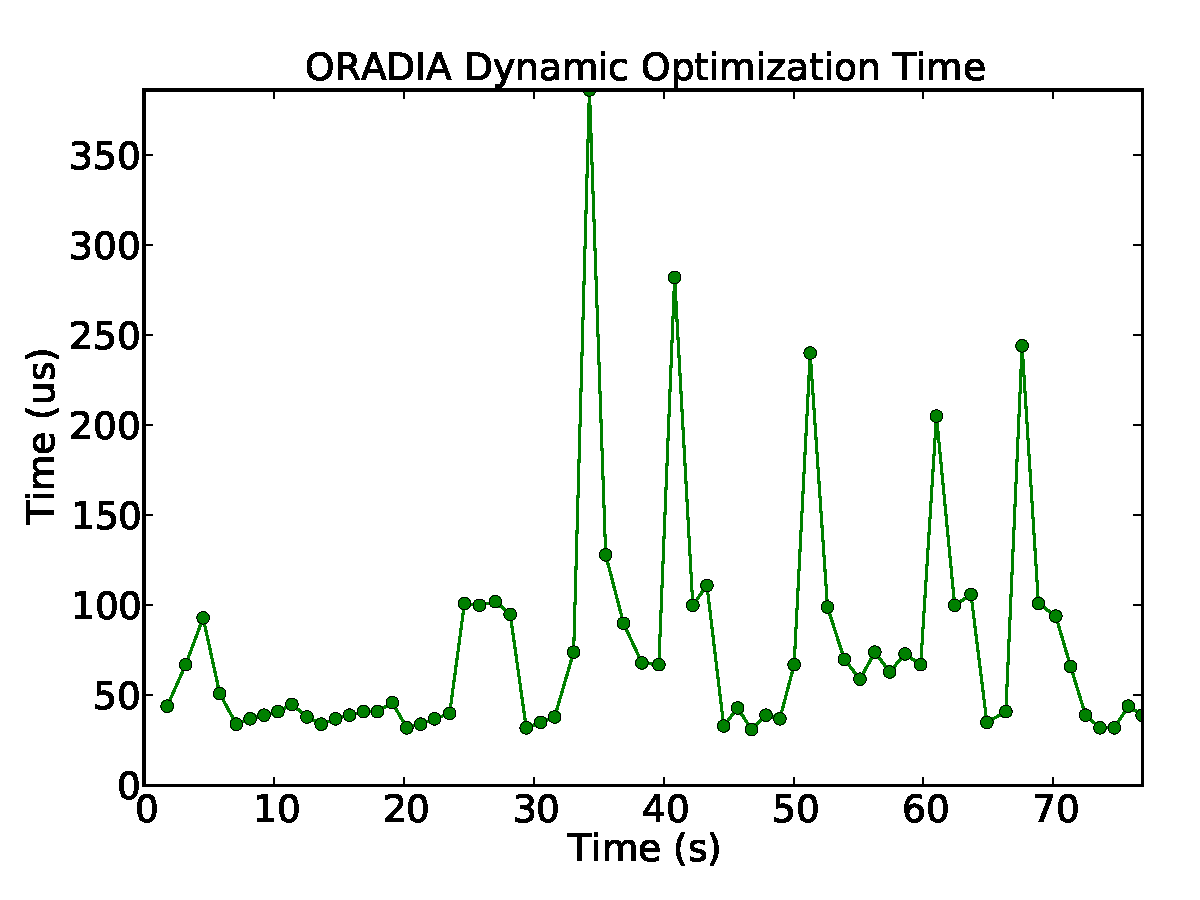
\includegraphics[bb=0 0 576 432,width=\columnwidth]{opt_time.pdf}
%%		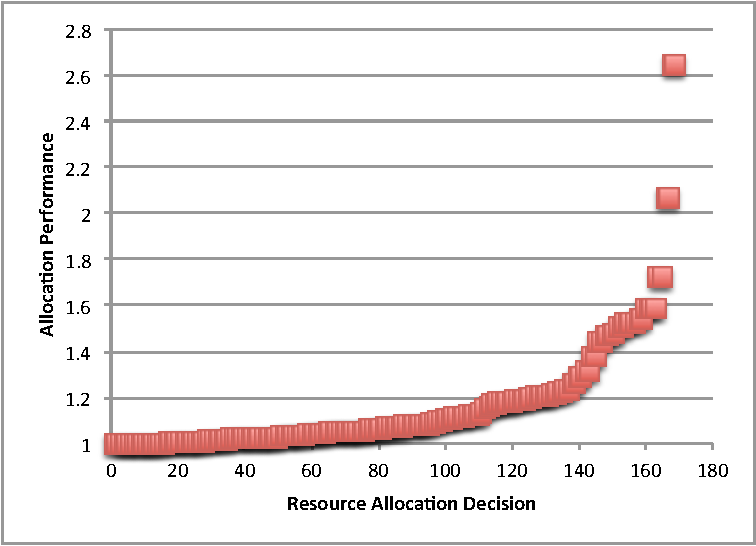
\includegraphics[width=.45\textwidth]{parsec_decision_points.pdf}
%		\caption{Performance of our penalty optimization algorithm}
%		\label{optimization_perf}
%	\end{center}
%\end{figure}


%Figure~\ref{optimization_perf} shows performance of the penalty optimization algorithm implemented in \tess.  

%For our video conferencing scenario the average runtime is \fix{x} and then worst case runtime is \fix{y}.  \fix{explain where the variance comes from}
